\documentclass[_main.tex]{subfiles}
 
\begin{document}

\section*{Population structure and migration}  \label{main_pop_struc}

So far we have treated the parasite population as a homogenous entity but it is more like a set of interconnnected subpopulations each inhabiting a particular geographical area.  There is spatial structure in transmission dynamics, e.g. neighbouring villages can vary in malaria prevalence due to differences in their mosquito breeding sites and other factors \cite{Bejon2010,Omedo2017}.  There is also a global population structure with genetic differentiation between continental regions, some of which reflects evolutionary adaptation to the resident vector and host populations \cite{Manske2012,MalariaGEN2023,Band2022}.

Essentially we have many \textit{local subpopulations} that are more or less loosely connected with each other and together make up a \textit{metapopulation}.  We could break this down into many different levels of spatial scale within a hierachical population structure, e.g.  local subpopulations could be embedded within regional metapopulations which are themselves embedded within the global metapopulation, as illustrated in figure \ref{fig:main_hierarchical_1}.  By convention, we use the subscript $_S$ to denote a local subpopulation and $_T$ to denote the total (or global) metapopulation. 

\begin{figure}[h!]
\centering
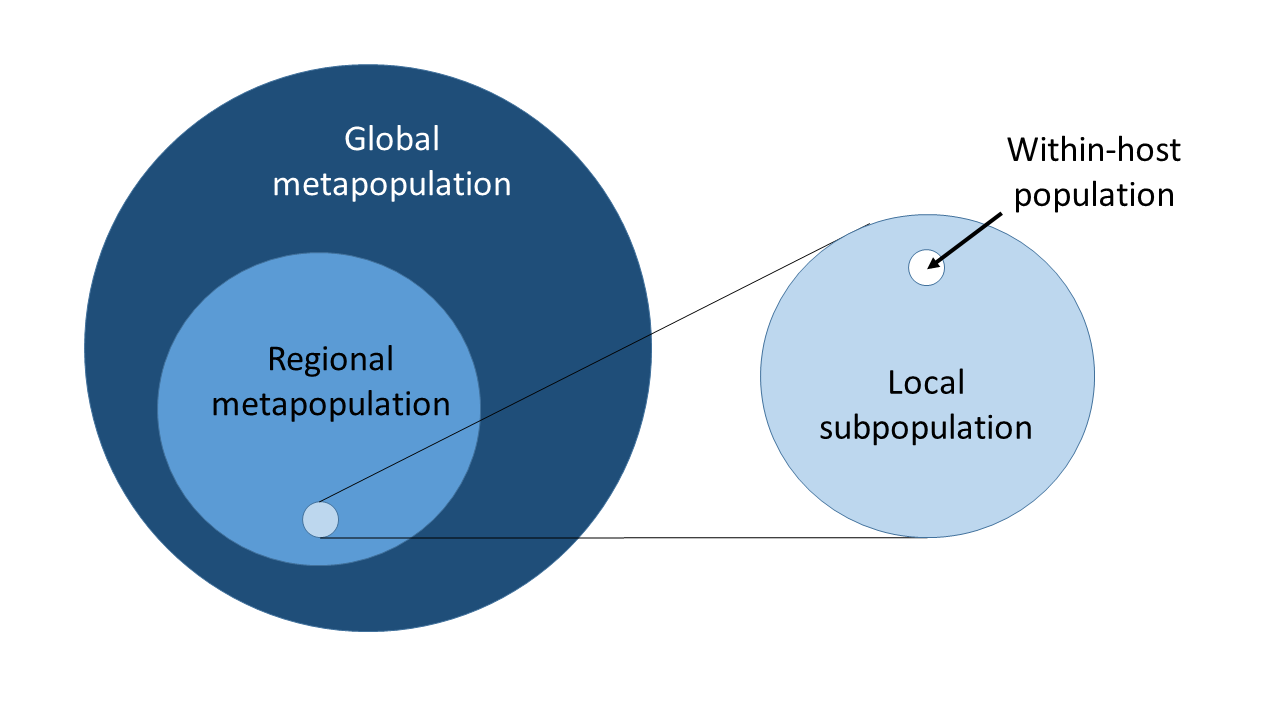
\includegraphics[width=10cm]{221112_hierarchical_pop_structure.png}
\caption{\textbf{Hierarchical population structure.}  Here we imagine that local subpopulations (e.g. villages) are embedded within much larger regional metapopulations (e.g. West Africa or Southeast Asia) which themselves are embedded within the global metapopulation.  The local subpopulation can itself be broken down into multiple within-host populations.}
\label{fig:main_hierarchical_1}
\end{figure}

\paragraph{Effect of global parasite dispersal on local population genetics.} Migration from the global metapopulation into a local subpopulation - either ongoing or due to historical patterns of global parasite dispersal - can have a profound effect on local population genetics.  To illustrate this let us consider the simple scenario of a local subpopulation within a much larger metapopulation.  

Let $m$ be the probability that a host within the local subpopulation acquired their infection from the metapopulation, and let the number of such hosts per generation be $N_m = m N_h$.  These migrant hosts could be either immigrants from the metapopulation or local residents who have been travelling outside the local area.  Methods section \ref{supp_trans_matrix_2} describes how we can work out the transmission probability matrix for the subpopulation, shown in table \ref{tab:tr_matrix_subpopulation}, while the transition probability matrix of the metapopulation is essentially as described in table \ref{tab:main_tr_matrix}.   

Table \ref{table:main_global_dispersal_1} illustrates the effects of migration on the nucleotide diversity of a local subpopulation ($N_h = 30$) embedded within a much larger metapopulation ($N_h = 3000$).   In the absence of migration, the nucleotide diversity of the subpopulation ($\pi_S = 2.4 \times 10^{-6}$) is two orders of magnitude lower than that of the metapopulation ($\pi_T = 3.7 \times 10^{-4}$).   With a migration rate of just one host every ten generations ($N_m = 0.1$) it increases dramatically ($\pi_S = 1.5 \times 10^{-4}$) and with a migration rate of one host per generation it is almost the same as the nucleotide diversity of the metapopulation.  

 \begin{table}[h!] 
\centering
\small{
\begin{tabular}{c c c c c c c c} 
\hline \\
$N_m$ & $\pi_T$ & $\pi_S$ & $\gamma_T$ & $\gamma_S$ & $F_{ST}$ \\ [0.5ex] 
\hline \\
0 & $3.7 \times 10^{-4} $ & $2.4 \times 10^{-6}$ & 0.004 & $0.41$ & $0.99$ \\ [2ex]
0.1 & $3.7 \times 10^{-4} $ &  $1.5 \times 10^{-4}$ & 0.004 & $0.32$ & $0.59$ \\ [2ex]
1 & $3.7 \times 10^{-4} $ &  $3.3 \times 10^{-4}$ & 0.004 & $0.10$ & $0.12$ \\ [2ex]
10 & $3.7 \times 10^{-4} $ &  $3.7 \times 10^{-4}$ & 0.004 & $0.01$ & $0.01$ \\ [2ex]
\hline
\end{tabular}
}
\caption{\small{\textbf{Effect of global dispersal on local genetic diversity.}  $N_m$ is the number of migrants per generation entering a local subpopulation ($N_h = 30, \chi = 0.5, Q = 10$) from a much larger global metapopulation ($N_h = 3000, \chi = 1, Q = 10$).   The table shows the nucleotide diversity of the metapopulation ($\pi_T$) and the subpopulation ($\pi_S$); the haplotype homozygosity of a 2cM locus in the metapopulation ($\gamma_T$) and the subpopulation ($\gamma_S$); and $F_{ST}$, the fixation index of the subpopulation relative to the metapopulation.  \href{https://d-kwiat.github.io/gtg/migration-simple.html}{See worked example.}}}
\label{table:main_global_dispersal_1}
\end{table}

We have already mentioned the evidence that current levels of nucleotide diversity in the global parasite population have built up over thousands of years, and here we see how relatively low levels of migration from the global metapopulation can cause a local subpopulation to achieve relatively high levels of between-host nucleotide diversity.  

\paragraph{Using fixation indices as a measure of hierarchical population structure.}  \label{main_fixation_indices}  In describing the effects of migration on population structure, it is helpful to use Wright's fixation index:

\begin{equation*}
F_{ST} = 1 - \frac{H_S}{H_T}
\end{equation*}

where $H_T$ is the heterozygosity of the total (or global) metapopulation and $H_S$ is the heterozygosity of a local subpopulation.  As shown in figure \ref{fig:main_migration_Fst}, $F_{ST}$ is inversely related to the rate of migration and the size of the local population.

\begin{figure}[h!]
\centering
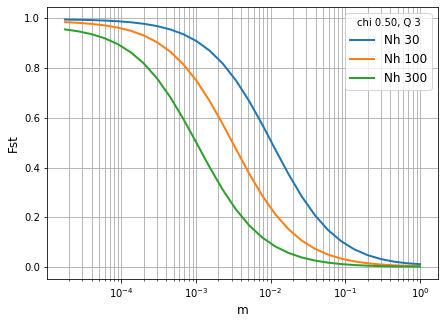
\includegraphics[width=8cm]{230127_Fst_m.png}
\caption{\textbf{Relationship between $F_{ST}$ and the rate of migration in a hierarchical population structure.}  We imagine a local subpopulation embedded within a metapopulation of $N_h = 3000, Q = 10, \chi = 1$.  $m$ is the probability that a host within the local subpopulation acquired their infection from the metapopulation. $F_{ST}$ is inversely related to $m$ and also to the size of the local population.
\href{https://github.com/d-kwiat/gtg/blob/main/migration_Fst.ipynb}{View code}
}
\label{fig:main_migration_Fst}
\end{figure}

\end{document}